\documentclass[12pt]{article}

\usepackage{graphicx,float,units,breqn}
\usepackage[font=footnotesize]{caption}

\newcommand{\ybar}{\overline{y}}

\begin{document}

%\begin{Large}
\noindent Mickey Warner
%\bigskip

\noindent Stat 651
%\end{Large}
\bigskip

\section{The 2001 Season for Barry Bonds}

\subsection{Summary}

\noindent The following is a Bayesian analysis of home runs and at-bats for former baseball player Barry Bonds during his 2001 season with the San Francisco Giants.  We take a close look at his home run percentage and provide several estimates to better understand his performance that year.

\subsection{The Likelihood and Conjugate Prior}

The probability density function comes from the binomial distribution, where $y_i$ is the number of home runs and $n_i$ is the number of at-bats in game $i$.  The function is defined as:

%\[f_*(y_i|\theta)={n_i \choose y_i}\theta^{y_i}(1-\theta)^{n_i-y_i}, 0<\theta<1, n_i=0,1,\cdots, y_i=0,1,\cdots,n_i\]

\begin{eqnarray*}
f_*(y_i|\theta)={n_i \choose y_i}\theta^{y_i}(1-\theta)^{n_i-y_i}; && 0\leq\theta\leq1; \\
&& n_i=0,1,\cdots; \\
&& y_i=0,1,\cdots,n_i \\
\end{eqnarray*}

\noindent The likelihood function is:

\begin{eqnarray*}
L(\mathbf{y}|\theta) &=& \prod_{i=1}^n\left[{n_i \choose y_i}\theta^{y_i}(1-\theta)^{n_i-y_i}\right] \\
&=& \left[\prod_{i=1}^n{n_i \choose y_i}\right]\theta^{\Sigma y_i}(1-\theta)^{\Sigma n_i-\Sigma y_i} \\
\end{eqnarray*}

\noindent For the prior we will use a beta distribution with parameters $a$ and $b$, which has the pdf
\[\pi(\theta)=\frac{\Gamma(a+b)}{\Gamma(a)\Gamma(b)}\theta^{a-1}(1-\theta)^{b-1}\ \ \ \ \ 0<\theta<1;\ a>0;\ b>0 \]

\noindent Solving for the posterior distribution will show that we have a conjugate prior.  This is accomplished by multiplying the likelihood and the prior together and diving by the integral of that product.

\begin{eqnarray*}
\pi(\theta|\mathbf{y}) &=& \frac{\left[\prod_{i=1}^n{n_i \choose y_i}\right]\theta^{\Sigma y_i}(1-\theta)^{\Sigma n_i-\Sigma y_i}\frac{\Gamma(a+b)}{\Gamma(a)\Gamma(b)}\theta^{a-1}(1-\theta)^{b-1}}{\int_0^1\left[\prod_{i=1}^n{n_i \choose y_i}\right]\theta^{\Sigma y_i}(1-\theta)^{\Sigma n_i-\Sigma y_i}\frac{\Gamma(a+b)}{\Gamma(a)\Gamma(b)}\theta^{a-1}(1-\theta)^{b-1}d\theta}  \\
\\
&=& \frac{\theta^{\Sigma y_i}(1-\theta)^{\Sigma n_i-\Sigma y_i}\theta^{a-1}(1-\theta)^{b-1}}{\int_0^1\theta^{\Sigma y_i}(1-\theta)^{\Sigma n_i-\Sigma y_i}\theta^{a-1}(1-\theta)^{b-1}d\theta} \\
\\
&=& \frac{\theta^{a+\Sigma y_i-1}(1-\theta)^{b+\Sigma n_i-\Sigma y_i-1}}{\int_0^1\theta^{a+\Sigma y_i-1}(1-\theta)^{b+\Sigma n_i-\Sigma y_i-1}d\theta} \\
\end{eqnarray*}

\noindent Let $a^*=a+\Sigma y_i$ and $b^*=b+\Sigma n_i-\Sigma y_i$, then

\begin{eqnarray*}
\pi(\theta|\mathbf{y}) &=& \frac{\theta^{a^*-1}(1-\theta)^{b^*-1}}{\int_0^1\theta^{a^*-1}(1-\theta)^{b^*-1}d\theta} \\
&=& \frac{\theta^{a^*-1}(1-\theta)^{b^*-1}}{\frac{\Gamma(a^*)\Gamma(b^*)}{\Gamma(a^*+b^*)}\int_0^1\frac{\Gamma(a^*+b^*)}{\Gamma(a^*)\Gamma(b^*)}\theta^{a^*-1}(1-\theta)^{b^*-1}d\theta} \\
&=& \frac{\theta^{a^*-1}(1-\theta)^{b^*-1}}{\frac{\Gamma(a^*)\Gamma(b^*)}{\Gamma(a^*+b^*)}} \\
&=& \frac{\Gamma(a^*+b^*)}{\Gamma(a^*)\Gamma(b^*)}\theta^{a^*-1}(1-\theta)^{b^*-1} \\
\end{eqnarray*}

\noindent which is a beta distribution with parameters $a^*=a+\Sigma y_i$ and $b^*=b+\Sigma n_i-\Sigma y_i$.  Thus, we have a conjugate prior.

\subsection{Prior Parameters}

\noindent Values for the priors were chosen to be $a=5$ and $b=45$.  When looking at Barry Bonds' record from the beginning of his career, we can see that his home run per at-bat percent has been gradually increasing from about 5\% in 1986 to about 10\% in 2000.  With the chosen priors we would have a mean of $\frac{5}{5+45}=10\%$.  Though we must be careful to have enough flexibility in these priors to adjust for the 2001 season, while still building off the previous years.
\bigskip

\noindent With a relatively high standard deviation of $\sqrt{\frac{(5)(45)}{(5+45)^2(5+45+1)}}=0.042$ we are more likely to take into account his performance in earlier years.  However, since his record has been improving, we do not want too much weight into these priors.  Having too high of priors could pull down our estimate calculated from the posterior distribution.  Thus values such as $a=10$ and $b=90$ were not selected, even though that distribution has a mean of $10\%$.  So $a=5$ and $b=45$ seem to be an appropriate choice.
\bigskip


\subsection{Maximum Likelihood and Plots}

%\noindent The plot for a Beta distribution with parameters $\alpha=5$ and $\beta=45$.

%\begin{figure}[H]
%\begin{center}
%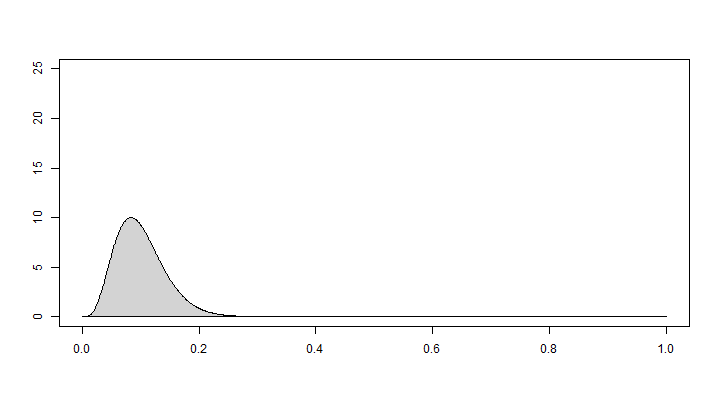
\includegraphics[scale=0.5]{figs/1priorplot.pdf}
%\caption{Prior distribution}
%\end{center}
%\end{figure}
%\bigskip
%\bigskip
%\bigskip

\noindent \textit{Parameters of the posterior distribution.}  In 2001, Barry Bonds was at-bat 476 times and hit 73 home runs.  Using this data to update our priors, we get posterior parameters of $a^*=5+73=78$ and $b^*=45+476-73=448$.
\bigskip

\noindent \textit{Derivation of the maximum likelihood estimator.}  First, take the logarithm of the likelihood.

\begin{eqnarray*}
\mathrm{log}L(y_i|\theta)&=& \mathrm{log}\left(\left[\prod_{i=1}^n{n_i \choose y_i}\right]\theta^{\Sigma y_i}(1-\theta)^{\Sigma n_i-\Sigma y_i}\right) \\
&=& \mathrm{log}\left[\prod_{i=1}^n{n_i \choose y_i}\right]+\Sigma y_i\mathrm{log}\theta+(\Sigma n_i-\Sigma y_i)\mathrm{log}(1-\theta) \\
\end{eqnarray*}

\noindent Then take the derivative.  

\begin{eqnarray*}
\frac{d}{d\theta}\left[\mathrm{log}L(y_i|\theta)\right] &=& 0 + \frac{\Sigma y_i}{\theta} - \frac{\Sigma n_i-\Sigma y_i}{1-\theta} \\
&=& \frac{\Sigma y_i}{\theta} - \frac{\Sigma n_i-\Sigma y_i}{1-\theta} \\
\end{eqnarray*}

\noindent Setting this equation equal to 0 and solving for $\hat{\theta}$ will give us our desired estimate.

\begin{eqnarray*}
0 &=& \frac{\Sigma y_i}{\hat{\theta}} - \frac{\Sigma n_i-\Sigma y_i}{1-\hat{\theta}}\\
\frac{\Sigma n_i-\Sigma y_i}{1-\hat{\theta}} &=& \frac{\Sigma y_i}{\hat{\theta}} \\
\hat{\theta}(\Sigma n_i-\Sigma y_i) &=& (1-\hat{\theta})\Sigma y_i \\
\hat{\theta}\Sigma n_i - \hat{\theta}\Sigma y_i &=& \Sigma y_i -\hat{\theta}\Sigma y_i \\
\hat{\theta}\Sigma n_i &=& \Sigma y_i \\
\hat{\theta} &=& \frac{\Sigma y_i}{\Sigma n_i} \\
\end{eqnarray*}

\noindent The MLE is calculated to be
\[\hat{\theta}=\frac{73}{476}=0.153.\]

\begin{figure}[H]
\begin{center}
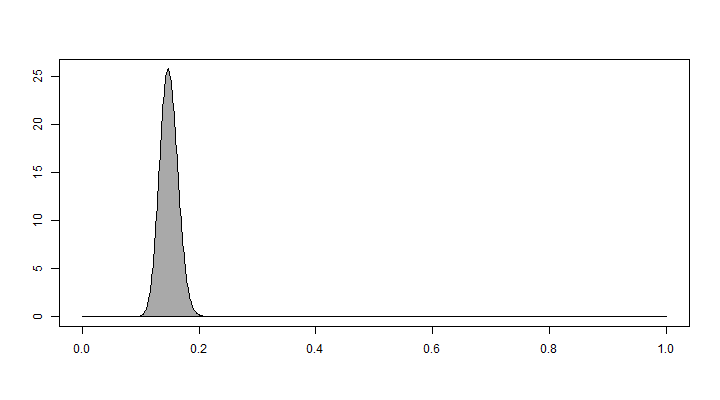
\includegraphics[scale=0.5]{figs/1postplot.pdf}
\caption{Plots of the prior (dashed), posterior (solid), and MLE (red).}
\end{center}
\end{figure}


\subsection{Posterior Estimates}

\begin{figure}[H]
\begin{center}
\begin{tabular}{l|r}
Estimate & \multicolumn{1}{l}{Value} \\ \hline \hline
Mean               & $0.1482$ \\
Median             & $0.1478$ \\
Mode               & $0.1469$ \\
Variance           & $0.0002$ \\
Standard Deviation & $0.0154$ \\
\end{tabular}
\end{center}
\end{figure}

\noindent The 95\% central credible interval is $(0.119, 0.179)$.

\subsection{Other Potential Priors}


\begin{figure}[H]
\begin{center}
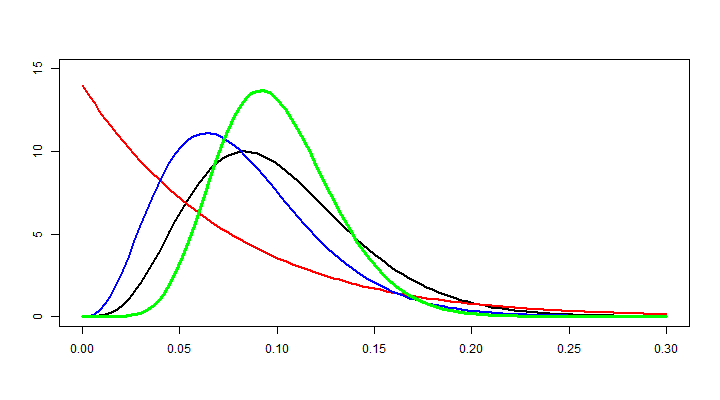
\includegraphics[scale=0.5]{figs/1otherpriors.pdf}
\caption{Four Posterior Distributions}
\end{center}
\end{figure}

\noindent \textit{Black}.  The priors used in the analysis $a=5$ and $b=45$.

\noindent \textit{Red}. $a=1$, $b=14$.  Based off all home runs and at-bats in seasons previous to 2001.  Very flexible to new data.

\noindent \textit{Blue}. $a=4$, $b=45$.  Looks only at the time Bonds was with the Giants before 2001.  Moderately flexible to new data.

\noindent \textit{Green}. $a=10$, $b=90$.  Uses only the 2000 season to select prior parameters.  New data affects posterior to a lesser degree than other priors.

%\subsection{Conclusion}
%
%In terms of home runs and at-bats, Barry Bonds did exceptionally well in 2001.  He averaged close to 15 home runs for every 100 at-bats.  The lower end of the 95\% credible interval suggests that with high probability Bonds played well enough to hit at least 11\% home runs.  There is also a good chance that he played well enough to hit up to 18\% home runs.  Considering only a handful of players have averaged more than 7\% home runs during their careers, Barry Bonds' 2001 season was indeed spectacular and significant.

\newpage

\section{Failures of the Fastest Computer in the World}

\subsection{Summary}

\noindent We will look at data for 15 months of failures of the Los Alamos National Laboratory ``fasted computer in the world.''  Experts say that the computer should not fail any more than 10 times in a month.

\subsection{The Likelihood and Conjugate Prior}

The probability density function comes from the Poisson distribution, where $y_i$ is the number of failures in a month.  The function, for $i=1,2,\cdots,15$, is:

\[f_*(y_i|\lambda)=\frac{\lambda^{y_i}e^{-\lambda}}{y_i!};\ \ \ \ \ \lambda\geq 0;\ y_i=0,1,\cdots \]

\noindent The likelihood function is:

\[L(\mathbf{y}|\lambda) = \prod_{i=1}^n\left(\frac{\lambda^{y_i}e^{-\lambda}}{y_i!}\right) = \frac{\lambda^{\Sigma y_i}e^{-n\lambda}}{\prod (y_i!)}\]

%\noindent The conjugate prior, as we shall see, is the Gamma distribution, which is:

%\[f(\lambda)=\frac{\beta^\alpha}{\Gamma(\alpha)}\lambda^{\alpha-1}e^{-\beta\lambda}\]

\noindent Using the gamma distribution (with the rate parametrization)

\[\pi(\lambda)=\frac{b^a}{\Gamma(a)}\lambda^{a-1}e^{-b\lambda};\ \ \ \ \ \lambda\geq 0;\ a,b>0\]

\noindent for our prior, we derive the posterior distribution

\begin{eqnarray*}
\pi(\lambda|\mathbf{y}) &=& \frac{\frac{\lambda^{\Sigma y_i}e^{-n\lambda}}{\prod (y_i!)}\frac{b^a}{\Gamma(a)}\lambda^{a-1}e^{-b\lambda}}{\int_0^\infty\frac{\lambda^{\Sigma y_i}e^{-n\lambda}}{\prod (y_i!)}\frac{b^a}{\Gamma(a)}\lambda^{a-1}e^{-b\lambda}d\lambda} \\
%&=& \frac{\lambda^{\Sigma y_i}e^{-n\lambda}\lambda^{\alpha-1}e^{-\beta\lambda}}{\int_0^\infty\lambda^{\Sigma y_i}e^{-n\lambda}\lambda^{\alpha-1}e^{-\beta\lambda}d\lambda} \\
&=& \frac{\lambda^{a+\Sigma y_i-1}e^{-\lambda(b+n)}}{\int_0^\infty\lambda^{a+\Sigma y_i-1}e^{-\lambda(b+n)}d\lambda} \\
&=& \frac{\lambda^{a+\Sigma y_i-1}e^{-\lambda(b+n)}}{\frac{\Gamma(a+\Sigma y_i)}{(b+n)^{a+\Sigma y_i}}\int_0^\infty\frac{(b+n)^{a+\Sigma y_i}}{\Gamma(a+\Sigma y_i)}\lambda^{a+\Sigma y_i-1}e^{-\lambda(b+n)}d\lambda} \\
&=& \frac{\lambda^{a+\Sigma y_i-1}e^{-\lambda(b+n)}}{\frac{\Gamma(a+\Sigma y_i)}{(b+n)^{a+\Sigma y_i}}} \\
&=& \frac{(b+n)^{a+\Sigma y_i}}{\Gamma(a+\Sigma y_i)}\lambda^{a+\Sigma y_i-1}e^{-\lambda(b+n)} \\
\end{eqnarray*}

\noindent which is a gamma distribution with parameters $a+\Sigma y_i$ and $b+n$.  %Thus we have a conjugate prior.

\subsection{Prior Parameters}

\noindent For this analysis, we chose priors of $a=18$ and $b=3$.  We consider the expert's statement that they thought there ``ought'' to be no more than 10 failures in one month.  There appears to be some uncertainty, even lack of confidence, from the expert.  For the most part, the expert's statement was believed and used as the basis in selecting the priors.
\bigskip

\noindent Such a choice would result in a mean and variance of $\frac{18}{3}=6$ in estimating $\lambda$.  The priors suggest that there is some probability ($0.39$) that the computer will fail more than 10 times in the month, but for the most part should agree with the expert's opinion.

\subsection{Maximum Likelihood and Plots}

%\noindent The plot for a Gamma distribution with parameters $\alpha=18$ and $\beta=3$.
%
%\begin{figure}[H]
%\begin{center}
%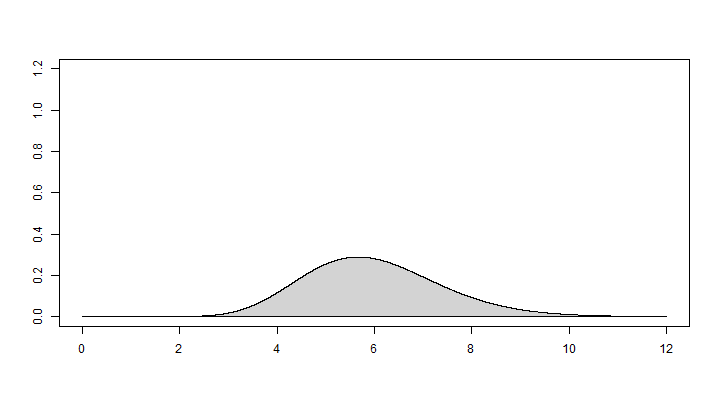
\includegraphics[scale=0.5]{figs/2priorplot.pdf}
%\caption{Prior Distribution}
%\end{center}
%\end{figure}

\noindent \textit{Parameters of the posterior distribution.}  From the data collected, there were a total of 34 failures in the 15 months.  So this means we have for posterior parameters $a^*=18+34=52$ and $b^*=3+15=18$.
\bigskip

\noindent \textit{Derivation of the maximum likelihood estimator.}  Take the logarithm of the likelihood function.

\begin{eqnarray*}
\mathrm{log}L(y_i|\lambda) &=& \mathrm{log}\left[\frac{\lambda^{\Sigma y_i}e^{-n\lambda}}{\prod (y_i!)}\right] \\
&=& \Sigma y_i\mathrm{log}\lambda-n\lambda-\mathrm{log}\prod (y_i!) \\
\end{eqnarray*}

\noindent Find the derivative of this with respect to $\lambda$.

\begin{eqnarray*}
\frac{d}{d\lambda}\left[\mathrm{log}L(y_i|\lambda)\right] &=& \frac{d}{d\lambda}\left[\Sigma y_i\mathrm{log}\lambda-n\lambda-\mathrm{log}\prod (y_i!)\right] \\
&=& \frac{\Sigma y_i}{\lambda}-n+0 \\
&=& \frac{\Sigma y_i}{\lambda}-n \\
\end{eqnarray*}

\noindent Set equal to 0 and solve for $\hat{\lambda}$.

\begin{eqnarray*}
0 &=& \frac{\Sigma y_i}{\hat{\lambda}}-n \\
%n &=& \frac{\Sigma y_i}{\hat{\lambda}} \\
\hat{\lambda} &=& \frac{\Sigma y_i}{n} \\
&=& \ybar \\
\end{eqnarray*}

\noindent which is evaluted to be $\hat{\lambda}=2.26$.

\begin{figure}[H]
\begin{center}
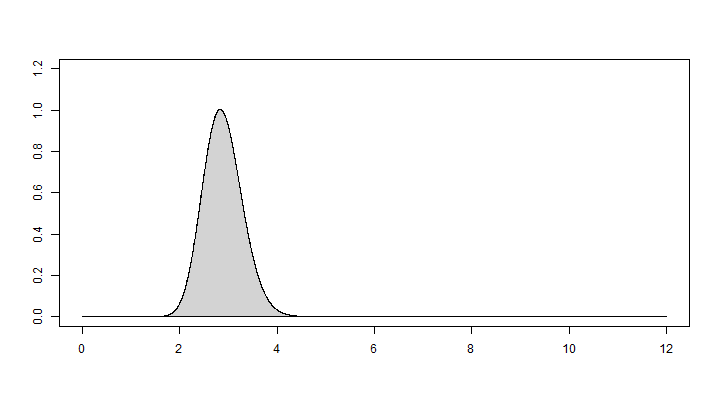
\includegraphics[scale=0.5]{figs/2postplot.pdf}
\caption{Plots of the prior (dashed), posterior (solid), and MLE (red).}
\end{center}
\end{figure}

\subsection{Posterior Estimates}

\begin{figure}[H]
\begin{center}
\begin{tabular}{l|r}
Estimator & \multicolumn{1}{l}{Value} \\ \hline \hline
Mean               & $2.88$ \\
Median             & $2.87$ \\
Mode               & $2.83$ \\
Variance           & $0.16$ \\
Standard Deviation & $0.40$ \\
\end{tabular}
\end{center}
\end{figure}

\noindent The 95\% central credible interval is $(2.15, 3.72)$.

\subsection{Other Potential Priors}

\begin{figure}[H]
\begin{center}
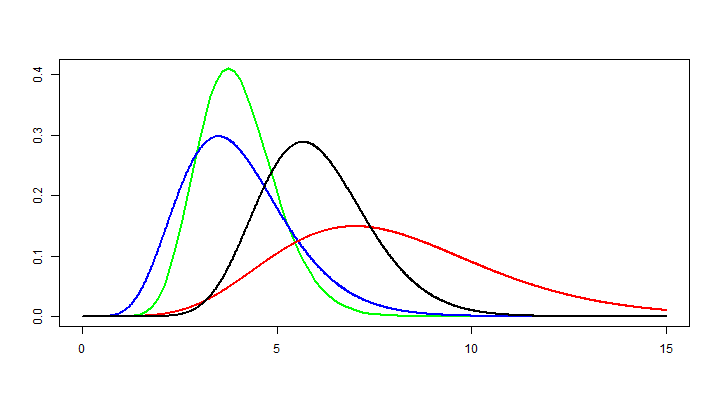
\includegraphics[scale=0.5]{figs/2otherpriors.pdf}
\caption{Four Posterior Distributions}
\end{center}
\end{figure}

\noindent \textit{Black}.  The priors used in the analysis $a=18$ and $b=3$.

\noindent \textit{Red}. $a=8$, $b=1$.  Not confident in experts response that the computer ``ought" not to fail more than 10 times a month.  Believes a value of 10 or higher is somewhat likely.

\noindent \textit{Blue}. $a=8$, $b=2$.  Most flexible to the data, but leans towards higher probability in lower amounts of failures.

\noindent \textit{Green}. $a=16$, $b=4$.  Has strong confidence in the experts.  Prior distribution has more weight in the posterior.


%\subsection{Conclusion}
%
%\noindent From our interval estimation we may say that there is a 95\% probability that $\lambda$ is not any less than 2.12 and no higher than 3.68.  Even at the higher end of the interval, having such a $\lambda$ would result in a minimal amount of months where the supercomputer failed 10 or more times.  Though there is still some chance of the computer failing that many times.
%\bigskip
%
%\noindent However, despite the possible occurrence of a high number of failures, using the estimates gathered from the posterior distribution we would realistically expect between 1 and 7 failures in any given month.  Collecting more data will allow us to construct narrower intervals and estimate $\lambda$ with greater accuracy.

\newpage

\section{North American Rivers}

\subsection{Summary}

\noindent We analyze the lengths (in miles) of 141 major rivers in North America.  It is common knowledge that the Mississippi river is one of the world's largest rivers, but this of course isn't typical of most of the major rivers in North America.  So how do river lengths on this continent compare to those around the world?

\subsection{The Likelihood and Conjugate Prior}

\noindent We assume the data is exponentially distributed.  The probability density function is:

\[f_*(y_i|\lambda)=\frac{1}{\lambda}e^{-y_i/\lambda} \]

\noindent The Likelihood function is:

\begin{eqnarray*}
L(y_i|\lambda) &=& \prod\left[\frac{1}{\lambda}e^{-y_i/\lambda}\right] \\
&=& \left(\frac{1}{\lambda}\right)^ne^{-\Sigma y_i/\lambda} \\
\end{eqnarray*}

\noindent We will use an Inverse Gamma distribution for the prior, which has pdf:

\[f(\lambda|a,b)=\frac{b^a}{\Gamma(a)}\left(\frac{1}{\lambda}\right)^{a+1}e^{-b/\lambda}\]

\noindent Multiplying the likelihood with the prior and dividing by the integral of that same product will give us the posterior distribution.  So we have

\begin{eqnarray*}
f(\lambda|y_i,a,b) &=& \frac{\left(\frac{1}{\lambda}\right)^ne^{-\Sigma y_i/\lambda}\frac{b^a}{\Gamma(a)}\left(\frac{1}{\lambda}\right)^{a+1}e^{-b/\lambda}}{\int_o^\infty \left(\frac{1}{\lambda}\right)^ne^{-\Sigma y_i/\lambda}\frac{b^a}{\Gamma(a)}\left(\frac{1}{\lambda}\right)^{a+1}e^{-b/\lambda}d\lambda} \\
&=& \frac{\left(\frac{1}{\lambda}\right)^{(a+n)+1}e^{-(b+\Sigma y_i)/\lambda}}{\int_0^\infty \left(\frac{1}{\lambda}\right)^{(a+n)+1}e^{-(b+\Sigma y_i)/\lambda}d\lambda} \\
&=& \frac{\left(\frac{1}{\lambda}\right)^{(a+n)+1}e^{-(b+\Sigma y_i)/\lambda}}{\frac{\Gamma(a+n)}{(b+\Sigma y_i)^{a+n}}\int_0^\infty \frac{(b+\Sigma y_i)^{a+n}}{\Gamma(a+n)}\left(\frac{1}{\lambda}\right)^{(a+n)+1}e^{-(b+\Sigma y_i)/\lambda}d\lambda} \\
&=& \frac{\left(\frac{1}{\lambda}\right)^{(a+n)+1}e^{-(b+\Sigma y_i)/\lambda}}{\frac{\Gamma(a+n)}{(b+\Sigma y_i)^{a+n}}} \\
&=& \frac{(b+\Sigma y_i)^{a+n}}{\Gamma(a+n)}\left(\frac{1}{\lambda}\right)^{(a+n)+1}e^{-(b+\Sigma y_i)/\lambda} \\
\end{eqnarray*}

\noindent which is an Inverse Gamma distribution with parameters $a^*=a+n$ and $b^*=b+\Sigma y_i$.  Therefore, the Inverse Gamma is the conjugate prior to the probability density function.
\bigskip

\begin{scriptsize}
\noindent \textit{Note:} In this analysis we are estimating $\lambda$.  The p.d.f., though a function $\lambda$, is in terms of $1/\lambda$.  This will turn out to be very convenient for us.  The p.d.f is an exponential distribution which has a mean and standard deviation of $1/\lambda$.  Thus with this particular function the mean and standard deviation will simply be $\lambda$.  So when we look at estimates of $\lambda$, we can easily make the connection between the parameter and what we are really interested in, i.e. river lengths in North America.
\end{scriptsize}

\subsection{Prior Parameters}

\noindent For our analysis we selected priors of $a=5$ and $b=1600$.  With an Inverse Gamma distribution, this means we have a mean of $\frac{b}{a-1}=400$ and standard deviation of $\sqrt{\frac{b^2}{(a-1)^2(a-2)}}=230.94$.
\bigskip

\noindent We want to choose priors that seem to match up with what we know about river lengths in North America (which is very little).  We are saying that the average length is about $400$ miles.  With a high standard deviation we have a higher chance of capturing the true mean in our analysis.  Since these priors are comparatively low, the posterior distribution will be more flexible to new data, which is what we want since we have little knowledge of anything about rivers.

\subsection{Maximum Likelihood and Plots}

The prior distribution with parameters $\alpha=5$ and $\beta=1600$.

\begin{figure}[H]
\begin{center}
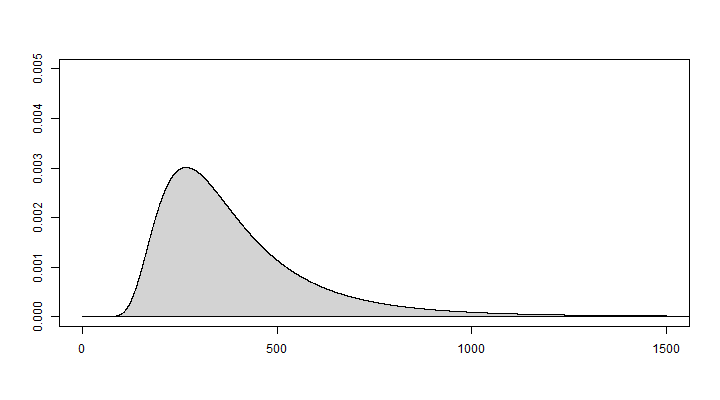
\includegraphics[scale=0.5]{figs/3priorplot.pdf}
\caption{Prior Distribution}
\end{center}
\end{figure}

\noindent With $n=141$ rivers and $\Sigma y_i=83357$, for the posterior distribution we have parameters $\alpha_1=5+141=146$ and $\beta_1=1600+83357=84957$.

\begin{figure}[H]
\begin{center}
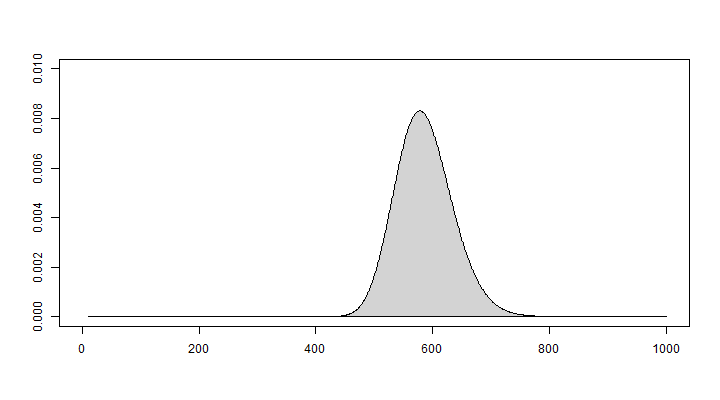
\includegraphics[scale=0.5]{figs/3postplot.pdf}
\caption{Posterior Distribution}
\end{center}
\end{figure}

\noindent \textit{Derivation of the maximum likelihood estimator.}  Begin, as before, by taking the logarithm of the likelihood function.

\begin{eqnarray*}
\mathrm{log}L(y_i|\lambda) &=& \mathrm{log}\left[\left(\frac{1}{\lambda}\right)^ne^{-\Sigma y_i/\lambda}\right] \\
&=& -n\mathrm{log}\lambda-\frac{\Sigma y_i}{\lambda} \\
\end{eqnarray*}

\noindent Find the derivative.

\begin{eqnarray*}
\frac{d}{d\lambda}\mathrm{log}L(y_i|\lambda) &=& \frac{d}{d\lambda}\left[-n\mathrm{log}\lambda-\frac{\Sigma y_i}{\lambda}\right] \\
&=& -\frac{n}{\lambda}+\frac{\Sigma y_i}{\lambda^2} \\
\end{eqnarray*}

\noindent Set equal to 0 and solve for $\hat{\lambda}$.

\begin{eqnarray*}
0 &=& -\frac{n}{\hat{\lambda}}+\frac{\Sigma y_i}{\hat{\lambda}^2} \\
\frac{n}{\hat{\lambda}} &=& \frac{\Sigma y_i}{\hat{\lambda}^2} \\
n\hat{\lambda} &=& \Sigma y_i \\
\hat{\lambda} &=& \frac{\Sigma y_i}{n} \\
&=& \ybar \\
\end{eqnarray*}

\subsection{Posterior Estimates}

\noindent Because there is no analytic solution to the median of an Inverse Gamma distribution, we took a large random sample and found the median of the sample.  Thus, our estimate for the median is an approximation and not exact.

\begin{figure}[H]
\begin{center}
\begin{tabular}{l|r}
Estimator & \multicolumn{1}{l}{Value} \\ \hline \hline
Mean               & $585.9$ \\
Median             & $583.2$ \\
Mode               & $577.9$ \\
Variance           & $2838.9$ \\
Standard Deviation & $48.8$ \\
\end{tabular}
\end{center}
\end{figure}

\noindent The highest posterior density interval is $(493.5, 683.5)$.

\subsection{Other Potential Priors}

\begin{figure}[H]
\begin{center}
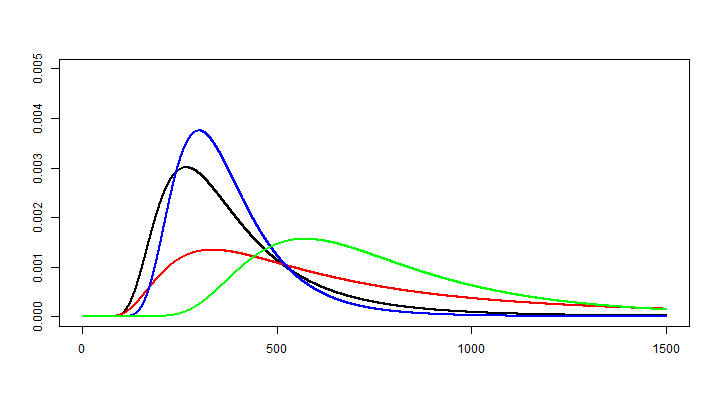
\includegraphics[scale=0.5]{figs/3otherpriors.pdf}
\caption{Four Posterior Distributions}
\end{center}
\end{figure}

\noindent \textit{Black}.  The priors used in the analysis $\alpha=5$ and $\beta=1600$.

\noindent \textit{Red}. $\alpha=2$, $\beta=1000$.  Most flexible to new data.  This was intended as the priors were chosen because of knowing little about North American rivers.

\noindent \textit{Blue}. $\alpha=9$, $\beta=3000$.  Attempts to agree with the lengths of the rivers in North America.  A brief internet search, independent of the data set, was used to get a rough estimate of the rivers.

\noindent \textit{Green}. $\alpha=6$, $\beta=4000$.  Priors based off a quick look at top river lengths throughout the world.  These parameters attempt to roughly match the mean from rivers worldwide.
\bigskip

\noindent Due to the large amount of data, it turns out that each of these choices in priors resulted in roughly the same posterior distribution.

%\subsection{Conclusion}
%
%\noindent We found that the posterior distribution for our parameter of interest $\lambda$ resulted in a mean of 585.  Credible interval bounds tells us that $\lambda$ has a 95\% probability of being within 493 and 683.  Now what we are interested in is what this tells us about river lengths in North America.  Conveniently enough, $\lambda$ corresponds with the mean length and standard deviation of rivers.  So the mean and standard deviation is $\lambda$.
%\bigskip
%
%\noindent The mode posterior distribution indicates to us that the most likely that $\lambda$ could be is 577.  That is, in North America, the average river length is 577.  Now these rivers follow an exponential distribution which has a very long tail, so we aren't surprised when rivers such as the Mississippi or Missouri show up in our data.  But most our river lengths will be around 600 miles or shorter.
%\bigskip
%
%\noindent Since this data came from North America's major rivers we would like to see how this compares to the world's major rivers.  Keep in mind that most rivers in North America will about no more than 600 or 650 miles long.  When considering the world's longest rivers, the river ranked 175th sits at about 645 miles.  So if we were to do an analysis on the world rivers, we would expect $\lambda$ to be somewhere close to 1000.  Not much of a competition for North America.

\newpage

\section{Statistics 221 Honors Students - (1)}

\subsection{Summary}

\noindent We analyze the test scores from the first exam in an honors section of Statistics 221.  This is an introductory course and we are told that the exam is ``extremely easy."

\subsection{The Likelihood and Conjugate Prior}

\noindent We will assume the data is normally distribution with mean $\mu$ and $\sigma=9$.  The probability density function is

\[f(y_i|\mu,\sigma)=(2\pi\sigma^2)^{-1/2}exp\left(-\frac{1}{2\sigma^2}(y_i-\mu)^2\right)\]

\noindent The likelihood function is

\begin{eqnarray*}
L(y_i|\mu,\sigma) &=& \prod\left[(2\pi\sigma^2)^{-1/2}exp\left(-\frac{1}{2\sigma^2}(y_i-\mu)^2\right)\right] \\
&=& (2\pi\sigma^2)^{-n/2}exp\left(-\frac{1}{2\sigma^2}\Sigma(y_i-\mu)^2\right) \\
\end{eqnarray*}

\noindent We will use a Normal distribution for the prior, assuming $\mu\sim N(\mu_0,\sigma_0^2)$.  The function for the prior is

\[f(\mu|\mu_0,\sigma_0^2)= (2\pi\sigma_0^2)^{-1/2}exp\left(-\frac{1}{2\sigma_0^2}(\mu-\mu_0)^2\right)\]

\noindent Since the posterior distribution is the likelihood times the prior divided by the integral of that product with respect to $\mu$, the full derivation would be too much to express all at once.  So we will look at only the numerator and cancel out any constants, which are any terms without $\mu$.  The posterior distribution is then

\begin{eqnarray*}
f(\mu|y_i,\sigma^2,\mu_0,\sigma_0^2) &\propto& (2\pi\sigma^2)^{\frac{-n}{2}}exp\left(\frac{-1}{2\sigma^2}\Sigma(y_i-\mu)^2\right)(2\pi\sigma_0^2)^{\frac{-1}{2}}exp\left(\frac{-1}{2\sigma_0^2}(\mu-\mu_0)^2\right) \\
&\propto& exp\left(-\frac{1}{2\sigma^2}\Sigma(y_i-\mu)^2\right)exp\left(-\frac{1}{2\sigma_0^2}(\mu-\mu_0)^2\right) \\
&\propto& exp\left(-\frac{1}{2\sigma^2}\Sigma(y_i-\mu)^2-\frac{1}{2\sigma_0^2}(\mu-\mu_0)^2\right) \\
&\propto& exp\left(-\frac{1}{2\sigma^2}(\Sigma y_i^2-2\mu\Sigma y_i+n\mu^2)-\frac{1}{2\sigma_0^2}(\mu^2-2\mu\mu_0+\mu_0^2)\right) \\
&\propto& exp\left(-\frac{1}{2\sigma^2\sigma_0^2}\left(\sigma_0^2(\Sigma y_i^2-2\mu\Sigma y_i+n\mu^2)+\sigma^2(\mu^2-2\mu\mu_0+\mu_0^2)\right)\right) \\
&\propto& exp\left(-\frac{1}{2\sigma^2\sigma_0^2}\left(\sigma_0^2(n\mu^2-2\mu\Sigma y_i)+\sigma^2(\mu^2-2\mu\mu_0)\right)\right) \\
&\propto& exp\left(-\frac{1}{2\sigma^2\sigma_0^2}\left(\sigma_0^2n\mu^2-\sigma_0^22\mu\Sigma y_i+\sigma^2\mu^2-\sigma^22\mu\mu_0\right)\right) \\
&\propto& exp\left(-\frac{1}{2\sigma^2\sigma_0^2}\left(\mu^2(\sigma_0^2n+\sigma^2)-2\mu(\sigma_0^2\Sigma y_i-\sigma^2\mu_0)\right)\right) \\
&\propto& exp\left[-\frac{1}{2\sigma^2\sigma_0^2}\left((\sigma_0^2n+\sigma^2)\left[\mu^2-2\mu\left(\frac{\sigma_0^2\Sigma y_i-\sigma^2\mu_0}{\sigma_0^2n+\sigma^2}\right)\right]\right)\right] \\
&\propto& exp\left[-\frac{\sigma_0^2n+\sigma^2}{2\sigma^2\sigma_0^2}\left(\mu^2-2\mu\left(\frac{\sigma_0^2n\ybar-\sigma^2\mu_0}{\sigma_0^2n+\sigma^2}\right)\right)\right] \\
\end{eqnarray*}

\noindent For simplicity in the remainder of the derivation we will let 

\[\psi=\frac{\sigma_0^2n\ybar-\sigma^2\mu_0}{\sigma_0^2n+\sigma^2}\]

\noindent which is a constant.

\begin{eqnarray*}
f(\mu|y_i,\sigma^2,\mu_0,\sigma_0^2) &\propto& exp\left[-\frac{\sigma_0^2n+\sigma^2}{2\sigma^2\sigma_0^2}\left(\mu^2-2\mu\psi\right)\right] \\
&\propto& exp\left[-\frac{\sigma_0^2n+\sigma^2}{2\sigma^2\sigma_0^2}\left(\mu^2-2\mu\psi+\psi^2-\psi^2\right)\right] \\
&\propto& exp\left[-\frac{\sigma_0^2n+\sigma^2}{2\sigma^2\sigma_0^2}\left(\mu^2-2\mu\psi+\psi^2\right)\right] \\
&\propto& exp\left(-\frac{1}{2(\frac{\sigma_0^2n+\sigma^2}{\sigma^2\sigma_0^2})}\left(\mu-\psi\right)^2\right) \\
\end{eqnarray*}

\noindent We now show that this is indeed a normal distribution.  Let

\[\tau^2=\frac{\sigma_0^2n+\sigma^2}{\sigma^2\sigma_0^2}\]

\noindent and show the full derivation.

\begin{eqnarray*}
f(\mu|y_i,\psi,\tau^2) &=& \frac{exp(-\frac{1}{2\tau^2}(\mu-\psi)^2)}{\int_{-\infty}^\infty exp(-\frac{1}{2\tau^2}(\mu-\psi)^2)d\mu} \\
&=& \frac{exp(-\frac{1}{2\tau^2}(\mu-\psi)^2)}{\frac{1}{(2\pi\tau^2)^{-\frac{1}{2}}}\int_{-\infty}^\infty(2\pi\tau^2)^{-\frac{1}{2}}exp(-\frac{1}{2\tau^2}(\mu-\psi)^2)d\mu} \\
&=& \frac{exp(-\frac{1}{2\tau^2}(\mu-\psi)^2)}{\frac{1}{(2\pi\tau^2)^{-\frac{1}{2}}}} \\
&=& (2\pi\tau^2)^{-\frac{1}{2}}exp\left(-\frac{1}{2\tau^2}(\mu-\psi)^2\right) \\
\end{eqnarray*}

\noindent This is a normal distribution with parameters $\psi=\frac{\sigma_0^2n\ybar-\sigma^2\mu_0}{\sigma_0^2n+\sigma^2}$ and $\tau^2=\frac{\sigma_0^2n+\sigma^2}{\sigma^2\sigma_0^2}$.  We may also write

\[\mathrm{Posterior}\sim N\left(\frac{\sigma_0^2n\ybar-\sigma^2\mu_0}{\sigma_0^2n+\sigma^2},\frac{\sigma_0^2n+\sigma^2}{\sigma^2\sigma_0^2}\right).\]

\noindent So we have our desired conjugate prior.

\subsection{Prior Parameters}

\noindent Since $\sigma^2$ is given and $\mu\sim N(\mu_0,\sigma_0^2)$ we only need to choose prior values for $\mu_0$ and $\sigma_0^2$.  We are told that the exam is extremely easy.  Since 70\% is typically thought of to be the average grade on a test, we will interpret ``extremely easy" to mean that the average is about 85\%, with some room for error.  So we will go with priors of $\mu_0=85$ and $\sigma_0^2=4$.
\bigskip

\subsection{Maximum Likelihood and Plots}

\noindent Parameters for the prior distribution are $\mu_0=85$ and $\sigma_0^2=4$.

\begin{figure}[H]
\begin{center}
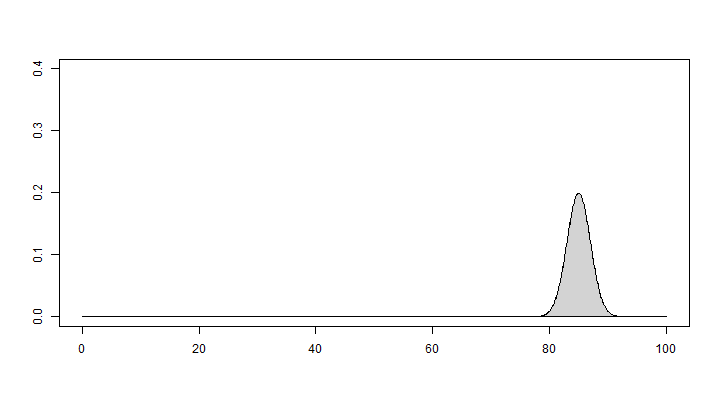
\includegraphics[scale=0.5]{figs/4priorplot.pdf}
\caption{Prior Distribution}
\end{center}
\end{figure}

\noindent Posterior distribution parameters: $\mu_1=86.34$ and $\sigma_1^2=1.64$.

\begin{figure}[H]
\begin{center}
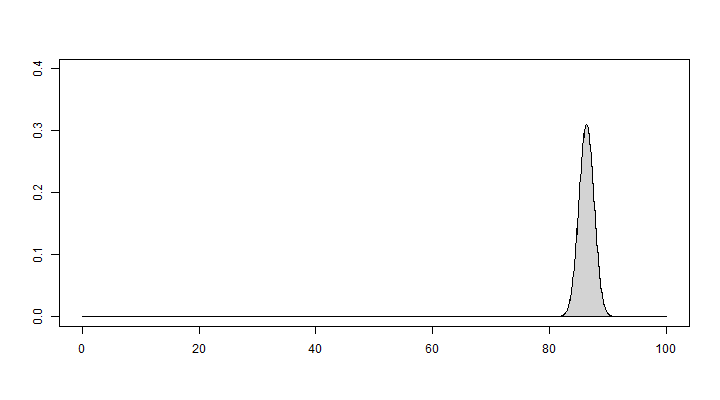
\includegraphics[scale=0.5]{figs/4postplot.pdf}
\caption{Posterior Distribution}
\end{center}
\end{figure}

\noindent \textit{Derivation of the maximum likelihood estimator.}  The log likelihood function for the normal distribution is:

\begin{eqnarray*}
\mathrm{log}L(y_i|\mu,\sigma^2) &=& \mathrm{log}\left[(2\pi\sigma^2)^{-n/2}exp\left(-\frac{1}{2\sigma^2}\Sigma(y_i-\mu)^2\right)\right] \\
&=& -\frac{n}{2}\mathrm{log}(2\pi\sigma^2)-\frac{1}{2\sigma^2}\Sigma(y_i-\mu)^2 \\
\end{eqnarray*}

The derivative with respect to $\mu$ is

\begin{eqnarray*}
\frac{d}{d\mu}\mathrm{log}L(y_i|\mu,\sigma^2) &=& \frac{d}{d\mu}\left[-\frac{n}{2}\mathrm{log}(2\pi\sigma^2)-\frac{1}{2\sigma^2}\Sigma(y_i-\mu)^2\right] \\
&=& -\frac{1}{2\sigma^2}\Sigma(y_i-\mu)(2)(-1) \\
&=& \frac{1}{\sigma^2}(\Sigma y_i-n\mu) \\
\end{eqnarray*}

Set equal to 0 and solve for $\hat{\mu}$

\begin{eqnarray*}
0 &=& \frac{1}{\sigma^2}(\Sigma y_i-n\hat{\mu}) \\
0 &=& (\Sigma y_i-n\hat{\mu}) \\
n\hat{\mu} &=& \Sigma y_i \\
\hat{\mu} &=& \frac{\Sigma y_i}{n} \\
&=& \ybar \\
\end{eqnarray*}

\subsection{Posterior Estimates}

\begin{figure}[H]
\begin{center}
\begin{tabular}{l|r}
Estimator & \multicolumn{1}{l}{Value} \\ \hline \hline
Mean               & $86.34$ \\
Median             & $86.34$ \\
Mode               & $86.34$ \\
Variance           & $1.64$ \\
Standard Deviation & $1.28$ \\
\end{tabular}
\end{center}
\end{figure}

\noindent The highest probability density interval is $(83.11, 89.56)$.


\subsection{Other Potential Priors}

\begin{figure}[H]
\begin{center}
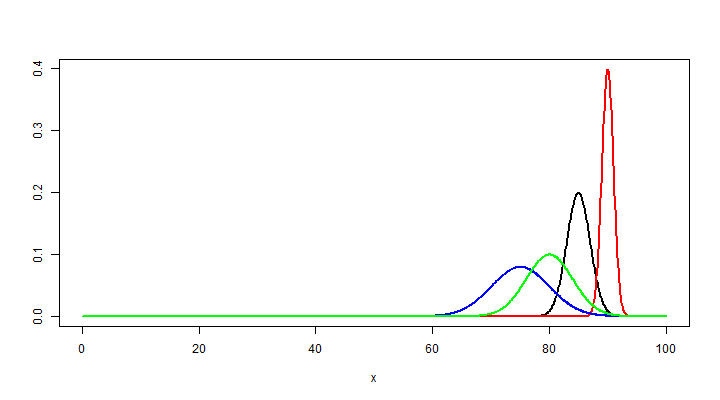
\includegraphics[scale=0.5]{figs/4otherpriors.pdf}
\caption{Four Posterior Distributions}
\end{center}
\end{figure}

\noindent \textit{Black}.  The priors used in the analysis $\mu_0=85$ and $\sigma_0^2=4$.

\noindent \textit{Red}. $\mu_0=90$, $\sigma_0^2=1$.  The justification of these priors comes from another interpretation of ``extremely easy" suggesting that the average test score is quite high.

\noindent \textit{Blue}. $\mu_0=75$, $\sigma_0^2=25$.  Higher variability in what the mean could be, but considers the average score to center around 75\%.

\noindent \textit{Green}. $\mu_0=80$, $\sigma_0^2=16$.  Similar to that used in the analysis, but with more variability.  This is to take into account a range of higher scores.

%\subsection{Conclusion}
%
%The analysis showed that the there is a 95\% probability that the average on the test score is between 83.1 and 89.5.  We normally think that an average grade on an exam should be about 70\%.  We may be tempted to agree with the test's description of extremely easy, but we should not forget that an honors section took the test.  Therefore it will be hard for us to conclude that the exam in reality is easy.  However, we are safe in saying, with good certainty as per the credible interval, that the mean is about 86.3\%.

\newpage

\section{Statistics 221 Honors Students - (2)}

\subsection{Summary}

\noindent We perform the same analysis as before, but this time we assume the data is distributed normally with parameters $\mu=87$ and unknown $\sigma$.  Therefore, we will be interested in estimating the variance.

\subsection{The Likelihood and Conjugate Prior}

\noindent The probability density function is

\[f(y_i|\mu,\sigma)=(2\pi\sigma^2)^{-1/2}exp\left(-\frac{1}{2\sigma^2}(y_i-\mu)^2\right)\]

\noindent The likelihood function is

\begin{eqnarray*}
L(y_i|\mu,\sigma) &=& \prod\left[(2\pi\sigma^2)^{-1/2}exp\left(-\frac{1}{2\sigma^2}(y_i-\mu)^2\right)\right] \\
&=& (2\pi\sigma^2)^{-n/2}exp\left(-\frac{1}{2\sigma^2}\Sigma(y_i-\mu)^2\right) \\
\end{eqnarray*}

\noindent We will use the Inverse Gamma distribution for the prior.  Let $\theta=\sigma^2$.  The posterior distribution is then

\begin{eqnarray*}
f(\theta|y_i,\mu,\alpha,\beta) &\propto& (2\pi\theta)^{-\frac{n}{2}}exp\left(-\frac{1}{2\theta}\Sigma(y_i-\mu)^2\right)\frac{\beta^\alpha}{\Gamma(\alpha)}\theta^{-\alpha-1}exp(-\beta/\theta) \\
&\propto& \theta^{-\frac{n}{2}}exp\left(-\frac{1}{2\theta}\Sigma(y_i-\mu)^2\right)\theta^{-\alpha-1}exp(-\beta/\theta) \\
&\propto& \theta^{-(\alpha+\frac{n}{2})-1}exp\left(-\frac{1}{\theta}\left(\frac{\Sigma(y_i-\mu)^2}{2}+\beta\right)\right) \\
\end{eqnarray*}

\noindent Let $\eta=\alpha+\frac{n}{2}$ and $\delta=\left(\frac{\Sigma(y_i-\mu)^2}{2}+\beta\right)$ then

\begin{eqnarray*}
f(\theta|y_i,\eta,\delta) &=& \frac{\theta^{-\eta-1}exp(-\delta/\theta)}{\int_0^\infty\theta^{-\eta-1}exp(-\delta/\theta)d\theta} \\
&=& \frac{\theta^{-\eta-1}exp(-\delta/\theta)}{\frac{\Gamma(\eta)}{\delta^\eta}\int_0^\infty\frac{\delta^\eta}{\Gamma(\eta)}\theta^{-\eta-1}exp(-\delta/\theta)d\theta} \\
&=& \frac{\theta^{-\eta-1}exp(-\delta/\theta)}{\frac{\Gamma(\eta)}{\delta^\eta}} \\
&=& \frac{\delta^\eta}{\Gamma(\eta)}\theta^{-\eta-1}exp(-\delta/\theta) \\
\end{eqnarray*}

\noindent This is an Inverse Gamma with parameters $\eta=\alpha+\frac{n}{2}$ and $\delta=\left(\frac{\Sigma(y_i-\mu)^2}{2}+\beta\right)$

\subsection{Prior Parameters}

\noindent Since we are given that $\mu=87$, we know we don't want a $\sigma^2$ that is too high since the max score is 100 and we would prefer not to go beyond that.  It seems appropriate to let a prior on $\sigma^2$ that causes the standard deviation to be about 6 or 7.  This means that two standard deviations above the mean will catch the max score and still go low enough to get the lower scores.  And since we are assuming the exam is easy, we wouldn't expect to go to for below the mean.

\subsection{Maximum Likelihood and Plots}

\noindent \textit{Derivation of the maximum likelihood estimator.}  Let $\theta=\sigma^2$ to avoid confusion in the derivative.  The log likelihood function is

\begin{eqnarray*}
\mathrm{log}L(y_i|\mu,\theta) &=& \mathrm{log}\left[(2\pi\theta)^{-n/2}exp\left(-\frac{1}{2\theta}\Sigma(y_i-\mu)^2\right)\right] \\
&=& -\frac{n}{2}\mathrm{log}(2\pi\theta)-\frac{1}{2\theta}\Sigma(y_i-\mu)^2 \\
\end{eqnarray*}

\noindent Take the derivative with respect to $\theta$

\begin{eqnarray*}
\frac{d}{d\theta}\mathrm{log}L(y_i|\mu,\theta) &=& \frac{d}{d\theta}\left[-\frac{n}{2}\mathrm{log}(2\pi\theta)-\frac{1}{2\theta}\Sigma(y_i-\mu)^2\right] \\
&=& -\frac{n}{2\theta}-\frac{1}{2\theta^2}\Sigma(y_i-\mu)^2(-1) \\
&=& -\frac{n}{2\theta}+\frac{1}{2\theta^2}\Sigma(y_i-\mu)^2 \\
\end{eqnarray*}

\noindent Set equal to 0 and solve for $\hat{\theta}=\hat{\sigma}^2$

\begin{eqnarray*}
0 &=& -\frac{n}{2\hat{\theta}}+\frac{1}{2\hat{\theta}^2}\Sigma(y_i-\mu)^2 \\
0 &=& -n\hat{\theta}+\Sigma(y_i-\mu)^2 \\
n\hat{\theta} &=& \Sigma(y_i-\mu)^2 \\
\hat{\sigma}^2=\hat{\theta} &=& \frac{\Sigma(y_i-\mu)^2}{n} \\
\end{eqnarray*}

\noindent Prior distribution with parameters $\alpha=2$ and $\beta=50$.

\begin{figure}[H]
\begin{center}
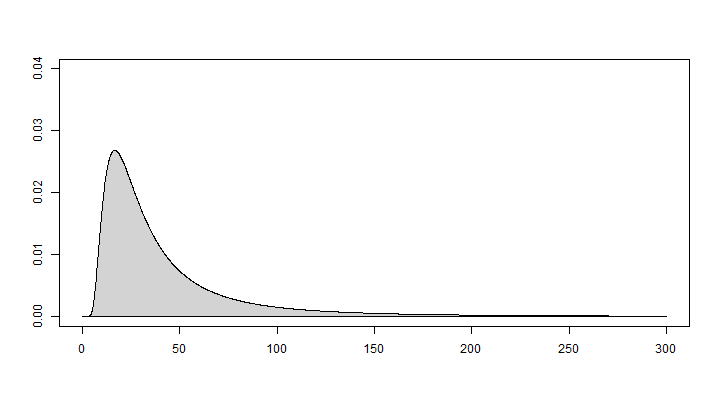
\includegraphics[scale=0.5]{figs/5priorplot.pdf}
\caption{Prior Distribution}
\end{center}
\end{figure}

\noindent Posterior distribution with parameters $\alpha_1=16.5$ and $\beta_1=1136$.

\begin{figure}[H]
\begin{center}
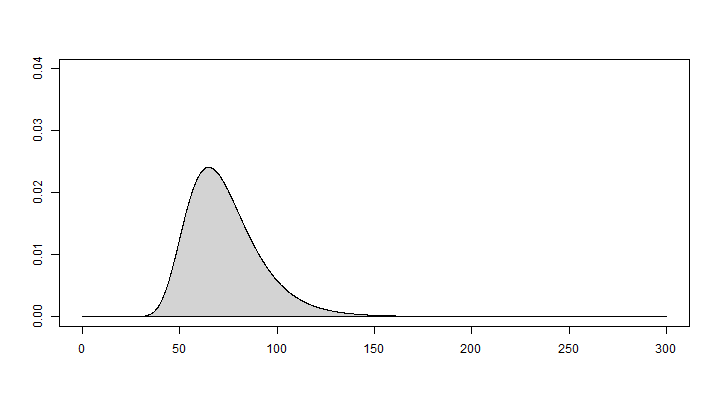
\includegraphics[scale=0.5]{figs/5postplot.pdf}
\caption{Posterior Distribution}
\end{center}
\end{figure}

\subsection{Posterior Estimates}

\begin{figure}[H]
\begin{center}
\begin{tabular}{l|r}
Estimator & \multicolumn{1}{l}{Value} \\ \hline \hline
Mean               & $73.2$ \\
Median             & $70.1$ \\
Mode               & $64.9$ \\
Variance           & $370.4$ \\
Standard Deviation & $19.2$ \\
\end{tabular}
\end{center}
\end{figure}

The highest probability density interval is $(41.4, 111.5)$.

\subsection{Other Potential Priors}

\begin{figure}[H]
\begin{center}
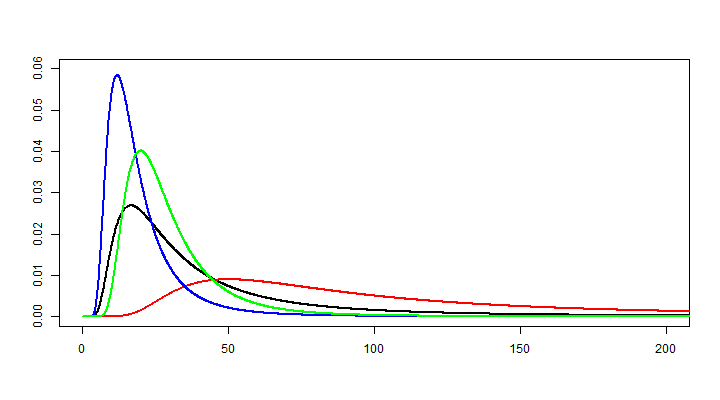
\includegraphics[scale=0.5]{figs/5otherpriors.pdf}
\caption{Four Posterior Distributions}
\end{center}
\end{figure}

\noindent \textit{Black}.  The priors used in the analysis $\alpha=2$ and $\beta=50$.

\noindent \textit{Red}. $\alpha=2$, $\beta=150$.  Variability is rather uncertain, so let it spread out further and be more flexible to new data.

\noindent \textit{Blue}. $\alpha=4$, $\beta=60$.  Presumes to be rather confident in choice of $\sigma^2$.  Priors have more weight, less flexible to new data.

\noindent \textit{Green}. $\alpha=5$, $\beta=120$.  Considers variability to be in a higher range, thinking that ``extremely easy" doesn't apply to all who took the test.

%\subsection{Conclusion}
%
%Taking the square root of our estimates will be most helpful in analyzing the distribution of the data.  For an HPD interval, we get $(6.44, 10.56)$ and this gives us a good idea of how our data are distributed.  In comparison to what we might normally expect with exam grades (say about 10), these standard deviations are small.  This suggests that, as a whole, the class did well and scored pretty close together, without too many low scores.

% \newpage
% 
% \section*{Appendix}
% 
% \subsection*{Part 1 Code}
% \begin{scriptsize}
% \begin{verbatim}
% ### Binomial with a Beta prior
% 
% path="C:/Users/Mickey/Desktop/Downloads/School/2013 A Winter/651/"
% bonds=read.table(paste(path,"binomial2.dat",sep=""))
% #V1 is date
% #V2 is number of at-bats in the game (n)
% #V3 is number of homeruns in the game (y)
% 
% priorA=5
% priorB=45
% 
% n=sum(bonds$V2)
% y=sum(bonds$V3)
% postA=priorA+y
% postB=priorB+n-y
% 
% pdf(paste(path,"1priorplot.pdf",sep=""),width=720,height=400)
% curve(dbeta(x,priorA,priorB),n=1001,ylim=c(0,25),
%     main="",
%     ylab="",xlab="")
% polygon(x=seq(0,1,0.001),
%     y=dbeta(seq(0,1,0.001),priorA,priorB),
%     col='lightgray',border='black')
% dev.off()
% 
% pdf(paste(path,"1postplot.pdf",sep=""),width=720,height=400)
% curve(dbeta(x,postA,postB),n=1001,main="",
%     ylab="",xlab="")
% polygon(x=seq(0,1,0.001),
%     y=dbeta(seq(0,1,0.001),postA,postB),
%     col='darkgray',border='black')
% dev.off()
% 
% ### Estimates
% #mean
% postA/(postA+postB)
% 
% #median
% qbeta(0.5,postA,postB)
% 
% #mode
% (postA-1)/(postA+postB-2)
% 
% #variance
% (postA*postB)/((postA+postB)^2*(postA+postB+1))
% 
% #standard deviation
% sqrt((postA*postB)/((postA+postB)^2*(postA+postB+1)))
% 
% # minimum interval approximation (HPD)
% n=10000
% p=0.95
% ints=matrix(NA,n,2)
% for (i in 0:(n-1)){
%     l=(1-p)/(n-1)*i
%     ints[i+1,1]=qbeta(l,postA,postB)
%     ints[i+1,2]=qbeta(l+p,postA,postB)
%     }
% len=ints[,2]-ints[,1]
% ints[which.min(len),]	#this is the approximation of the narrowest interval
% min(len)
% 
% ### Other priors
% # mean closer to that of all previous seasons, lighter weights
% a1=1
% b1=14
% 
% # only takes into account when bonds was with the giants 1993 - 2000, medium weights
% a2=4
% b2=45
% 
% # only data from 2000 season used, stronger weights
% a3=10
% b3=90
% 
% pdf(paste(path,"1otherpriors.pdf",sep=""),width=720,height=400)
% curve(dbeta(x,priorA,priorB),lwd=2,xlim=c(0,0.3),ylim=c(0,15),
%     main="",xlab="",ylab="")
% curve(dbeta(x,a1,b1),lwd=2,col='red',add=T)
% curve(dbeta(x,a2,b2),lwd=2,col='blue',add=T)
% curve(dbeta(x,a3,b3),lwd=3,col='green',add=T)
% dev.off()
% \end{verbatim}
% \end{scriptsize}
% 
% \subsection*{Part 2 Code}
% \begin{scriptsize}
% \begin{verbatim}
% ### Poisson with a Gamma prior
% 
% path="C:/Users/Mickey/Desktop/Downloads/School/2013 A Winter/651/"
% 
% comps=read.table(paste(path,"poisson.dat",sep=""))
% comps=t(comps)
% 
% priorA=18
% priorB=3
% 
% postA=priorA+sum(comps)
% postB=priorB+length(comps)
% 
% pdf(paste(path,"2priorplot.pdf",sep=""),width=720,height=400)
% curve(dgamma(x,priorA,priorB),n=1001,xlim=c(0,12),
%     main="",ylab="",xlab="",ylim=c(0,1.2))
% polygon(x=seq(0,12,0.001),
%     y=dgamma(seq(0,12,0.001),priorA,priorB),
%     col='lightgray',border='black')
% dev.off()
% 
% pdf(paste(path,"2postplot.pdf",sep=""),width=720,height=400)
% curve(dgamma(x,postA,postB),n=1001,xlim=c(0,12),
%     main="",ylab="",xlab="",ylim=c(0,1.2))
% polygon(x=seq(0,12,0.001),
%     y=dgamma(seq(0,12,0.001),postA,postB),
%     col='lightgray',border='black')
% dev.off()
% 
% ### Estimates
% 
% #mean
% postA/postB
% 
% #median
% qgamma(0.5,postA,postB)
% 
% #mode
% (postA-1)/postB
% 
% #variance
% postA/postB^2
% 
% #standard deviation
% sqrt(postA/postB^2)
% 
% #highest posterior density interval
% 
% n=10000
% p=0.95
% ints=matrix(NA,n,2)
% for (i in 0:(n-1)){
%     l=(1-p)/(n-1)*i
%     ints[i+1,1]=qgamma(l,postA,postB)
%     ints[i+1,2]=qgamma(l+p,postA,postB)
%     }
% len=ints[,2]-ints[,1]
% ints[which.min(len),]	#this is the approximation of the narrowest interval
% min(len)
% 
% 
% # Other priors
% 
% pdf(paste(path,"2otherpriors.pdf",sep=""),width=720,height=400)
% curve(dgamma(x,16,4),add=FALSE,col='green',xlim=c(0,15),lwd=2,
%     main="",xlab="",ylab="")
% curve(dgamma(x,8,2),n=1001,add=TRUE,col='blue',lwd=2)
% curve(dgamma(x,8,1),n=1001,add=TRUE,col='red',lwd=2)
% curve(dgamma(x,18,3),n=1001,add=TRUE,col='black',lwd=2)
% dev.off()
% \end{verbatim}
% \end{scriptsize}
% 
% \subsection*{Part 3 Code}
% \begin{scriptsize}
% \begin{verbatim}
% ### Exponential with an Inverse Gamma prior
% 
% path="C:/Users/Mickey/Desktop/Downloads/School/2013 A Winter/651/"
% 
% river=read.table(paste(path,"exponential.dat",sep=""))
% river=t(river)
% 
% igpdf=function(x,alpha,beta){
%     ((beta^alpha)/(gamma(alpha)))*(1/x)^(alpha+1)*exp(-beta/x)
% }
% 
% ### since the data make the gamma function and the beta^alpha 
% ### very large, we quickly reach to either 0 or infinity at any
% ### value of x.  So "ig2pdf" takes all the multiplications in the pdf
% ### separately, making the big numbers smaller and preventing
% ### errors in reaching to 0 or infinity to quickly.
% ig2pdf=function(x,alpha,beta){
%     out=beta
%     toA=1
%     toB=0
%     for (a in 1:(alpha-1)){
%         out=out/(alpha-a)
%         if (toB<ceiling(1*beta/3)){
%             out=out*exp(-1/x)
%             toB=toB+1
%             }
%         if (toA<ceiling(1*alpha/3)){
%             out=out*beta
%             toA=toA+1
%             }
%         }
%     for (a in 1:(alpha+1)){
%         out=out*(1/x)
%         if (toB<ceiling(2*beta/3)){
%             out=out*exp(-1/x)
%             toB=toB+1
%             }
%         if (toA<ceiling(2*alpha/3)){
%             out=out*beta
%             toA=toA+1
%             }
%         }
%     for (ab in 1:max(alpha,beta)){
%         if (toB<ceiling(beta)){
%             out=out*exp(-1/x)
%             toB=toB+1
%             }
%         if (toA<ceiling(alpha)){
%             out=out*beta
%             toA=toA+1
%             }
%         }
%     return(out)
%     }
% 
% 
% ### the gamma function gets too big so it freaks out,
% ### try a metropolis sampler
% 
% priorA=5
% priorB=1600
% 
% postA=priorA+length(river)
% postB=priorB+sum(river)
% 
% pdf(paste(path,"3priorplot.pdf",sep=""),width=720,height=400)
% xx=seq(0,1800,.1)
% plot(xx,igpdf(xx,priorA,priorB),xlim=c(0,1500),
%     main="",ylab="",xlab="",ylim=c(0,0.005),type='l')
% polygon(x=xx,
%     y=igpdf(xx,priorA,priorB),
%     col='lightgray',border='black')
% dev.off()
% 
% pdf(paste(path,"3postplot.pdf",sep=""),width=720,height=400)
% xx=seq(0,1000,1)
% plot(xx,ig2pdf(xx,postA,postB),xlim=c(0,1000),
%     main="",ylab="",xlab="",ylim=c(0,0.01),type='l')
% polygon(x=xx,
%     y=ig2pdf(xx,postA,postB),
%     col='lightgray',border='black')
% dev.off()
% 
% ### Estimates
% samp=1/rgamma(10000,postA,postB)
% 
% #mean
% postB/(postA-1)
% 
% #median
% quantile(samp,0.5)
% 
% #mode
% postB/(postA+1)
% 
% #variance
% (postB^2)/(((postA-1)^2)*(postA-2))
% 
% #standard deviation
% sqrt((postB^2)/(((postA-1)^2)*(postA-2)))
% 
% #highest posterior density interval
% 
% n=5000
% p=0.95
% ints=matrix(NA,n,2)
% for (i in 0:(n-1)){
%     l=(1-p)/(n-1)*i
%     ints[i+1,1]=quantile(samp,l)
%     ints[i+1,2]=quantile(samp,l+p)
%     }
% len=ints[,2]-ints[,1]
% ints[which.min(len),]	#this is the approximation of the narrowest interval
% min(len)
% 
% # Other priors
% 
% pdf(paste(path,"3otherpriors.pdf",sep=""),width=720,height=400)
% xx=seq(0,1500,.1)
% plot(xx,igpdf(xx,5,1600),xlim=c(0,1500),
%     main="",ylab="",xlab="",ylim=c(0,0.005),type='l',lwd=2)
% lines(xx,igpdf(xx,2,1000),lwd=2,col='red')
% lines(xx,igpdf(xx,9,3000),lwd=2,col='blue')
% lines(xx,igpdf(xx,6,4000),lwd=2,col='green')
% dev.off()
% \end{verbatim}
% \end{scriptsize}
% 
% \subsection*{Part 4 Code}
% \begin{scriptsize}
% \begin{verbatim}
% ### Normal (unknown mean) with Normal prior
% 
% path="C:/Users/Mickey/Desktop/Downloads/School/2013 A Winter/651/"
% 
% exammu=read.table(paste(path,"normalmean.dat",sep=""))
% exammu=t(exammu)
% 
% priorA=85
% priorB=4
% sigma2=81
% 
% n=length(exammu)
% ybar=mean(exammu)
% 
% postA=(n*ybar*priorB+priorA*sigma2)/(n*priorB+sigma2)
% postB=(sigma2*priorB)/(n*priorB+sigma2)
% 
% pdf(paste(path,"4priorplot.pdf",sep=""),width=720,height=400)
% xx=seq(0,100,.1)
% curve(dnorm(x,priorA,sqrt(priorB)),from=0,to=100,n=1000,main="",
%     xlab="",ylab="",ylim=c(0,0.4))
% polygon(x=xx,
%     y=dnorm(xx,priorA,sqrt(priorB)),
%     col='lightgray',border='black')
% dev.off()
% 
% pdf(paste(path,"4postplot.pdf",sep=""),width=720,height=400)
% xx=seq(0,100,.1)
% curve(dnorm(x,postA,sqrt(postB)),from=0,to=100,n=1000,main="",
%     xlab="",ylab="",ylim=c(0,0.4))
% polygon(x=xx,
%     y=dnorm(xx,postA,sqrt(postB)),
%     col='lightgray',border='black')
% dev.off()
% 
% #mean/median/mode
% postA
% 
% #variance
% postB
% 
% #standard deviation
% sqrt(postB)
% 
% #highest posterior density interval
% qnorm(c(0.025,0.975),postA,postB)
% 
% # Other priors
% 
% pdf(paste(path,"4otherpriors.pdf",sep=""),width=720,height=400)
% curve(dnorm(x,85,sqrt(4)),xlim=c(0,100),n=1000,main="",ylab="",
%     ylim=c(0,0.4),type='l',lwd=2)
% curve(dnorm(x,90,sqrt(1)),type='l',col='red',add=T,lwd=2,n=1000)
% curve(dnorm(x,75,sqrt(25)),type='l',col='blue',add=T,lwd=2,n=1000)
% curve(dnorm(x,80,sqrt(16)),type='l',col='green',add=T,lwd=2,n=1000)
% dev.off()
% \end{verbatim}
% \end{scriptsize}
% 
% \subsection*{Part 5 Code}
% \begin{scriptsize}
% \begin{verbatim}
% ### Normal (unknown variance) with an Inverse Gamma prior
% 
% path="C:/Users/Mickey/Desktop/Downloads/School/2013 A Winter/651/"
% 
% examvar=read.table(paste(path,"normalvariance.dat",sep=""))
% examvar=t(examvar)
% 
% igpdf=function(x,alpha,beta){
%     ((beta^alpha)/(gamma(alpha)))*(1/x)^(alpha+1)*exp(-beta/x)
% }
% 
% ig2pdf=function(x,alpha,beta){
%     out=beta
%     toA=1
%     toB=0
%     for (a in 1:(alpha-1)){
%         out=out/(alpha-a)
%         if (toB<ceiling(1*beta/3)){
%             out=out*exp(-1/x)
%             toB=toB+1
%             }
%         if (toA<ceiling(1*alpha/3)){
%             out=out*beta
%             toA=toA+1
%             }
%         }
%     for (a in 1:(alpha+1)){
%         out=out*(1/x)
%         if (toB<ceiling(2*beta/3)){
%             out=out*exp(-1/x)
%             toB=toB+1
%             }
%         if (toA<ceiling(2*alpha/3)){
%             out=out*beta
%             toA=toA+1
%             }
%         }
%     for (ab in 1:max(alpha,beta)){
%         if (toB<ceiling(beta)){
%             out=out*exp(-1/x)
%             toB=toB+1
%             }
%         if (toA<ceiling(alpha)){
%             out=out*beta
%             toA=toA+1
%             }
%         }
%     return(out)
%     }
% 
% 
% ### the gamma function gets too big so it freaks out,
% ### try a metropolis sampler
% 
% priorA=2
% priorB=50
% mu=87
% 
% postA=priorA+length(examvar)/2
% postB=priorB+0.5*sum((examvar-mu)^2)
% 
% pdf(paste(path,"5priorplot.pdf",sep=""),width=720,height=400)
% xx=seq(0,300,.1)
% plot(xx,igpdf(xx,priorA,priorB),xlim=c(0,300),
%     main="",ylab="",xlab="",ylim=c(0,0.04),type='l')
% polygon(x=c(xx,300),
%     y=c(igpdf(xx,priorA,priorB),0),
%     col='lightgray',border='black')
% dev.off()
% 
% pdf(paste(path,"5postplot.pdf",sep=""),width=720,height=400)
% xx=seq(0,300,.1)
% plot(xx,igpdf(xx,postA,postB),xlim=c(0,300),
%     main="",ylab="",xlab="",ylim=c(0,0.04),type='l')
% polygon(x=c(xx,300),
%     y=c(igpdf(xx,postA,postB),0),
%     col='lightgray',border='black')
% dev.off()
% 
% ### Estimates
% samp=1/rgamma(10000,postA,postB)
% 
% #mean
% postB/(postA-1)
% 
% #median
% quantile(samp,0.5)
% 
% #mode
% postB/(postA+1)
% 
% #variance
% (postB^2)/(((postA-1)^2)*(postA-2))
% 
% #standard deviation
% sqrt((postB^2)/(((postA-1)^2)*(postA-2)))
% 
% #highest posterior density interval
% 
% n=5000
% p=0.95
% ints=matrix(NA,n,2)
% for (i in 0:(n-1)){
%     l=(1-p)/(n-1)*i
%     ints[i+1,1]=quantile(samp,l)
%     ints[i+1,2]=quantile(samp,l+p)
%     }
% len=ints[,2]-ints[,1]
% ints[which.min(len),]
% min(len)
% 
% # Other priors
% 
% pdf(paste(path,"5otherpriors.pdf",sep=""),width=720,height=400)
% xx=seq(0,500,.1)
% plot(xx,igpdf(xx,2,50),xlim=c(0,200),
%     main="",ylab="",xlab="",ylim=c(0,0.06),type='l',lwd=2)
% lines(xx,igpdf(xx,2,150),lwd=2,col='red')
% lines(xx,igpdf(xx,4,60),lwd=2,col='blue')
% lines(xx,igpdf(xx,5,120),lwd=2,col='green')
% dev.off()
% \end{verbatim}
% \end{scriptsize}

\end{document}
